% !TeX program = xelatex
% Simin. General layout adapted from Sheng Li's Shanghai University Beamer template.
% 主文件 slide.tex；使用 XeLaTeX；本地可执行 latexmk -xelatex slide.tex。
\documentclass[UTF8,fontset=fandol]{ctexbeamer}
\usepackage{SHU}
\AtBeginSection[]{}
\AtBeginSubsection[]{}

% 方括号填写页脚简称，花括号填写封面信息。
\title[鞅与停时]{高等概率论：鞅与停时}
\subtitle{离散时间的可选停止定理\\[.25em]Martingales and Optional Stopping}
\author[Simin]{Simin}
\institute[上海大学]{上海大学}
\date[高等概率论]{高等概率论课程讲义}
\titlegraphic{
\includegraphics[height=1.12cm]{pic/SHU.png}}
\newcommand{\E}{\mathbb{E}}
\newcommand{\Prob}{\mathbb{P}}
\newcommand{\F}{\mathcal{F}}

\begin{document}

% 封面保留中央校徽与三栏页脚。分组使正文从下一页恢复浅灰角标。
{\logo{}
\begin{frame}
  \titlepage
\end{frame}
}

\section{鞅与停时}

\begin{frame}{从 2 出发，先到 5 的概率是多少？}
  一枚公平硬币决定每一步的方向。正面向上走一格，反面向下走一格，
  各次投掷相互独立。首次到达 0 或 5 时结束。
  \[
      X_0=2,\qquad X_n=2+\sum_{k=1}^{n}\xi_k,\qquad
      \Prob(\xi_k=1)=\Prob(\xi_k=-1)=\tfrac12 .
  \]
  \begin{block}{边界命中概率}
    若终点只有 0 和 5，知道终点的期望就能算出先到 5 的概率。
    在到达边界的一刻，位置的期望还等于 2 吗？
  \end{block}
\end{frame}

\begin{frame}{鞅：已知过去，下一步的期望在哪里？}
  令 $\F_n=\sigma(\xi_1,\ldots,\xi_n)$ 表示前 $n$ 次投掷提供的信息，
  $\F_0$ 为平凡 $\sigma$-代数。随着观测增加，$\F_n\subseteq\F_{n+1}$。
  \begin{block}{离散时间鞅}
    对每个 $n$，若 $M_n$ 是 $\F_n$-可测的，$\E|M_n|<\infty$，且
    \[
      \E[M_{n+1}\mid\F_n]=M_n\quad\text{几乎处处},
    \]
    则称 $(M_n)$ 是关于 $(\F_n)$ 的鞅。\cite{williams}
  \end{block}
  对公平随机游走，增量独立于过去且均值为零，因此
  $\E[X_{n+1}\mid\F_n]=X_n$。
\end{frame}

\begin{frame}{停时：首次碰到边界时停下}
  令 $\tau=\inf\{n\geq 0:X_n\in\{0,5\}\}$。
  观察到第 $n$ 步，就能判断 $\{\tau\leq n\}$ 是否发生。
  这正是停时条件 $\{\tau\leq n\}\in\F_n$。
  \begin{center}
    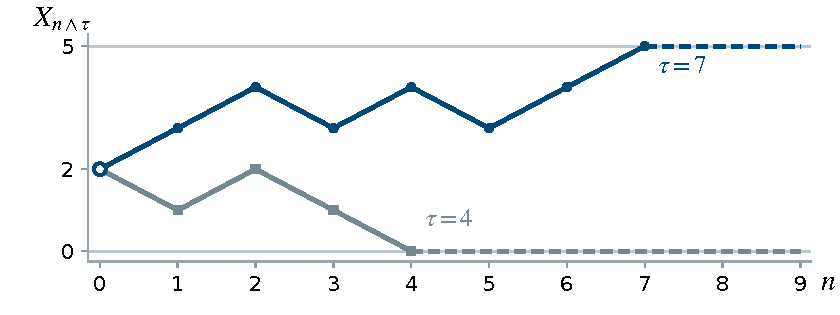
\includegraphics[width=.87\textwidth,height=.44\textheight,keepaspectratio]{pic/sample.pdf}
  \end{center}
  \small 图中的两条路径分别在第 4 步和第 7 步首次到达边界。
  虚线表示停止过程 $X_{n\wedge\tau}$ 此后保持终值。
\end{frame}

\section{可选停止定理}

\begin{frame}{有界停时的可选停止定理}
  \begin{block}{定理}
    设 $(M_n)$ 是离散时间鞅，$T$ 是停时。若存在确定整数 $N$，
    使得 $0\leq T\leq N$ 几乎处处，则 $\E[M_T]=\E[M_0]$。\cite{durrett}
  \end{block}
  将停止位置写成各步增量之和：
  \[
     M_T-M_0=\sum_{k=1}^{N}
       \mathbf{1}_{\{T\geq k\}}(M_k-M_{k-1}).
  \]
  $\{T\geq k\}\in\F_{k-1}$，而给定 $\F_{k-1}$ 时第 $k$ 步增量的条件期望为零。
  对每项取期望，再相加即得结论。
\end{frame}

\begin{frame}{从有界截断回到首次命中时刻}
  $\tau$ 可以超过任意固定步数。先取 $T_n=\tau\wedge n$，
  由有界停时定理可得 $\E[X_{T_n}]=2$。
  \begin{enumerate}
    \item \textbf{最终会停。} 从任何内部位置出发，接下来连续四步向上
      就一定触及上界。因此 $\Prob(\tau>4k)\leq(15/16)^k\to0$。
    \item \textbf{可以取极限。} $X_{T_n}\to X_\tau$ 几乎处处，且
      $0\leq X_{T_n}\leq5$。由支配收敛定理，
      \[
        \E[X_\tau]=\lim_{n\to\infty}\E[X_{T_n}]=2 .
      \]
  \end{enumerate}
\end{frame}

\begin{frame}{先到达 5 的概率为五分之二}
  记 $p=\Prob(X_\tau=5)$。由于步长为 1，终点恰好落在两个边界之一，
  \[
    2=\E[X_\tau]=0\,(1-p)+5p,
    \qquad \boxed{p=\tfrac{2}{5}} .
  \]
  \begin{exampleblock}{换一个起点}
    对同样的公平游走，若边界为 $0$ 和正整数 $b$，从整数 $i$ 出发
    （$0<i<b$），相同的截断论证给出先到达 $b$ 的概率 $i/b$。
  \end{exampleblock}
\end{frame}

\begin{frame}{参考文献}
  \bibliographystyle{plain}
  \bibliography{ref}
\end{frame}
\end{document}
